\subsubsection{\stid{1.14} UPC++} 
\paragraph{Overview} 
The Lightweight Communication and Global Address Space Support project (Pagoda)
is developing UPC++~\cite{upcxx-site}, a C++ library
supporting Partitioned Global Address Space (PGAS) programming~\cite{upcxx-ipdps19,upcxx-spec}.
The current UPC++ v1.0 (distinct from an earlier prototype designated V0.1
\cite{zheng:ipdps14}) is distinguished by three guiding principles.
First, all communication is \emph{asynchronous}, allowing overlap of computation and
communication, and encouraging programmers to avoid global synchronization. Second, all communication
is \emph{syntactically explicit}, encouraging programmers to consider the costs of communication. Third,
UPC++ encourages the use of \emph{scalable data-structures},
avoiding non-scalable library features.
These principles provide a programming model that can
scale efficiently to potentially millions of processors.
UPC++ is well-suited for implementing elaborate distributed data structures where
communication is irregular or fine-grained. 
The UPC++ communication interfaces for Remote Memory Access (RMA) 
and Remote Procedure Calls (RPC)
are composable and fit naturally within the context of modern C++.

UPC++ is needed for ECP because it delivers low-overhead communication,
embracing interest by vendors in the PGAS model to
efficiently match RDMA capabilities of modern
network hardware and on-chip communication between distinct address
spaces.  
Because ECP applications rely on irregular representations
to improve accuracy and conserve memory, the UPC++ library provides
an essential ingredient for the ECP software stack.  It enables
effective scaling of exascale software by reducing the work funneled
to lightweight cores, avoiding the overhead of long, branchy serial
code paths, and providing efficient fine-grained communication.  The
importance of these properties is reinforced by application trends;
many ECP applications require the use of irregular data structures such as 
adaptive meshes, sparse
matrices, particles, or similar techniques, and also perform load balancing.  UPC++'s
low-overhead communication mechanisms can maximize injection rate and
network utilization, tolerate latency through overlap, streamline
unpredictable communication events, minimize synchronization,
leverage hardware support for communication involving accelerator memory,
and efficiently support small- to medium-sized messages arising in such
applications.  UPC++ enables the ECP software stack to exploit
the best-available communication mechanisms, including novel features
being developed by vendors.
UPC++ provides seamless and efficient multithreading support,
offering a complementary and
interoperable approach to ``MPI + X'', enabling developers to
focus their effort on optimizing performance-critical communication.

\paragraph{Key  Challenges}

As a result of technological trends, the cost of data motion is steadily increasing relative to that of computation.  To reduce communication costs we need to 
reduce the software overheads and hide communication latency behind available computation. UPC++ addresses both strategies.
UPC++ avoids the software overheads associated with MPI, 
instead relying on the GASNet-EX~\cite{gasnet-site,gasnet-lcpc18}
communication library which is specifically designed and tuned
for native PGAS communication using the best-available hardware
mechanisms on each network
(see Section~\ref{subsubsect:gasnet-ex} on GASNet-EX, which is being co-designed).
UPC++ supports asynchronous communication via one-sided RMA and RPC.

\paragraph{Solution Strategy}

The UPC++ project has two primary thrusts:

% Non-use of a enumerated environment is intentional, due to excessive whitespce

\textbf{1. Increased performance through reduced communication costs:} The
UPC++ programmer can expect communication to run at close to hardware speeds.
Asynchronous execution enables an application to hide communication behind
available computation.

\textbf{2. Improved productivity:}  UPC++'s treatment of asynchronous
execution relies on futures and promises, and these simplify the management of
asynchrony.

The PGAS one-sided RMA communication employed by UPC++
benefits application  performance by mapping tightly onto the RDMA mechanisms
supported by the network hardware. GASNet-EX provides the
thin middleware
needed to enable this model to run at close to hardware speeds, across platforms ranging from laptops to supercomputers.
One-sided communication also has another benefit:
it decouples synchronization from data motion,
avoiding the fine-grained synchronization overheads of message-passing.

UPC++'s Remote Procedure Call (RPC)
enables the programmer
to execute procedure calls on remote processors.
RPC is useful in managing access to complicated irregular data structures,
and in expressing asynchronous task execution, where communication patterns
are data-dependent and hence difficult to predict.

As one example of how our approach is applicable to real problems
we have implemented a distributed hash table, which serves as a proxy
for a key phase in the HipMer application of the Exabiome Project (WBS~2.2.4.04).
This implementation scales efficiently
to a large number of processors. RPC was observed to simplify the implementation
considerably, by avoiding data hazards without the need for locking.
Figure~\ref{fig:dht} illustrates the benefits of the UPC++ model 
in a weak scaling study up to 34,816 processes on the KNL partition of NERSC's Cori.


\begin{wrapfigure}[17]{L}{.44\linewidth}
  \vspace{-1.5em}
  \centering
      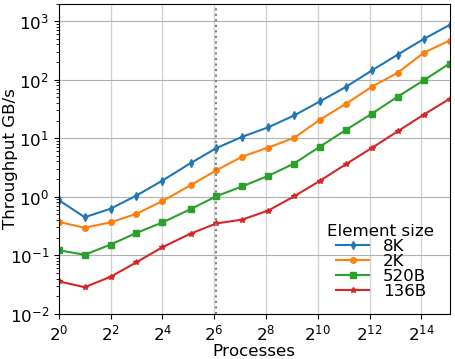
\includegraphics[scale=0.70]{projects/2.3.1-PMR/2.3.1.14-UPCxx-GASNet/all-cori-knl-out-inserts-wait.png}
  \caption{Weak scaling of distributed hash table insertion on the KNL partition of NERSC's Cori platform. The dotted line represents one node.}
  \label{fig:dht}
\end{wrapfigure}


\vspace{-2em}
\paragraph{Recent Progress}

The most notable work in the past year has been in three areas:

\textbf{1. Memory Kinds.}
UPC++ ``memory kinds'' provide a unified abstraction for communication between
combinations of device (e.g. GPU) and host memory, possibly remote.  By
unifying the expression of data transfer among the various memories in a
heterogeneous system, these abstractions enable ECP
applications to utilize accelerators within UPC++'s PGAS model.  The
abstraction enables hardware offload (when available) of device data transfers,
eliminating the need for the application to stage transfers through
intermediate buffers in host memory.
The global pointer representation transparently tracks device information,
eliminating the need for expensive address space queries in critical paths.
Support for such offload on the OLCF's
Summit has been demonstrated in an October 2020 memory kinds prototype
distributed to our stakeholders.

\textbf{2. Training and Outreach.}
In the past year, the UPC++ team has increased focus on outreach.  This includes
presenting four training events, and preparation of a fifth to appear at SC20.
A two-hour ``Birds of a Feather'' event in August 2020 introduced current and
potential UPC++ users to the authors of successful UPC++-based applications.
Circulation of working group drafts of proposed enhancements has
been valuable to both the UPC++ team and our stakeholders to agree upon design
in advance of implementation.

\textbf{3. Productivity and Performance.}
Having completed the core specification and implementation of UPC++, we have
shifted focus toward addressing improvements to productivity and performance,
especially in response to stakeholder feedback.  The most significant
example is addition of support for non-trivial serialization of
user-defined types, providing concise syntax for the common cases and
robust, extensible mechanisms for more complex ones.

\paragraph{Next Steps}

The planned work for the near-term future includes the following:

\textbf{1. Memory Kinds.}
We will continue development of the October 2020 memory kinds prototype.  The
implementation, currently targeting the hardware in Summit, will be extended to
include other accelerators scheduled to appear in the early Exascale systems.
As with Summit, transfers will be offloaded to available hardware capabilities
by leveraging the parallel efforts in GASNet-EX.

\textbf{2. Productivity and Performance.}
With the help of our stakeholders, we will continue to identify and address
portions of UPC++ where performance tuning is most needed
and/or beneficial.  Similarly, we will continue to work with stakeholders to
identify and implement features which improve productivity.

\textbf{3. Outreach.}
We will continue to hold training events for users of UPC++ and circulate
working group drafts of productivity features (above) to solicit feedback.
